% flashcards-title: Translate a position-time curve to velocity
% flashcards-desc: A concave-down position-time curve is followed by three candidate velocity-time graphs: increasing through zero, decreasing through zero, and decreasing while remaining positive.
\documentclass[border=7pt]{standalone}
\def\pgfsysdriver{pgfsys-dvisvgm.def}
\usepackage{tikz}
\usetikzlibrary{arrows.meta,positioning,shapes.geometric}
\definecolor{mechInk}{HTML}{172033}
\definecolor{mechBlue}{HTML}{155EEF}
\definecolor{mechOrange}{HTML}{B54708}
\definecolor{mechPale}{HTML}{E8F0FF}
\definecolor{mechGray}{HTML}{667085}
\definecolor{mechLight}{HTML}{D0D5DD}
\tikzset{
  every picture/.style={font=\sffamily\large, text=mechInk},
  mech box/.style={draw=mechInk, line width=1.2pt, rounded corners=4pt,
    fill=white, align=center, minimum height=14mm, inner xsep=5mm},
  mech primary/.style={draw=mechBlue, line width=2.2pt},
  mech secondary/.style={draw=mechOrange, line width=2.2pt, dashed},
  mech guide/.style={draw=mechGray, line width=0.9pt, dashed},
  mech arrow/.style={-{Stealth[length=3.2mm,width=2.4mm]},
    draw=mechInk, line width=1.4pt, line cap=butt},
  mech axis/.style={draw=mechInk, line width=1.2pt},
  mech tick/.style={draw=mechInk, line width=1pt}
}

\begin{document}
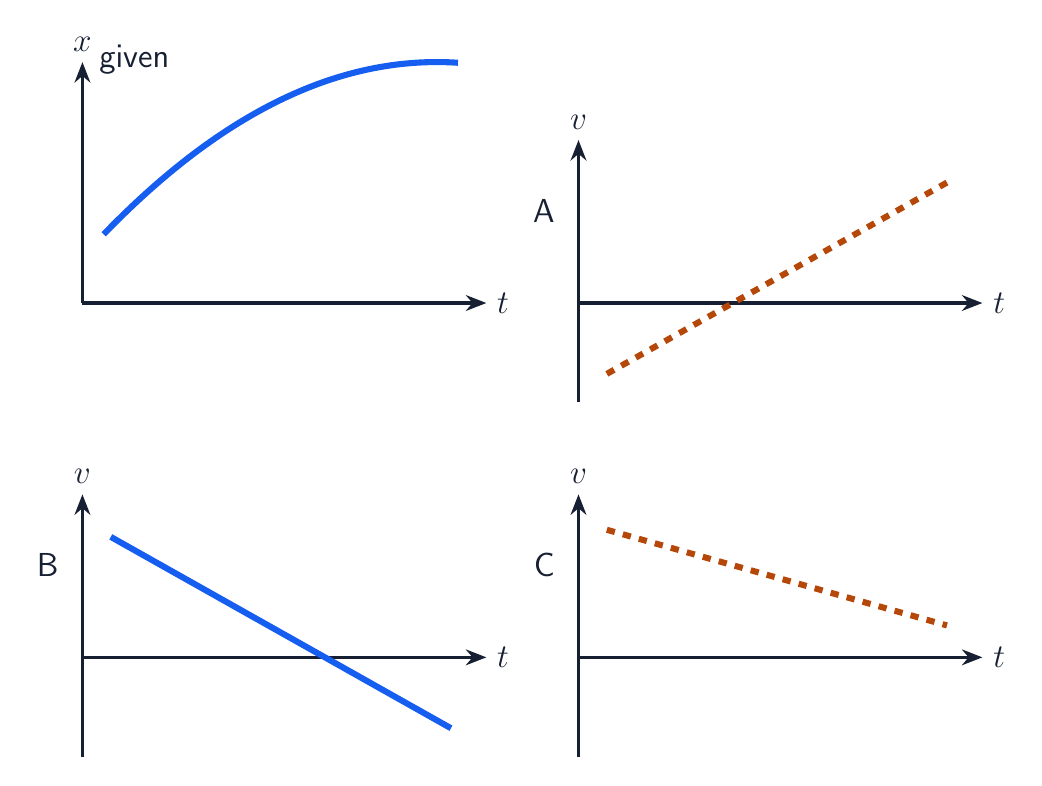
\begin{tikzpicture}[x=0.9cm,y=0.9cm]
  \begin{scope}[shift={(0,5)}]
    \draw[mech axis,-{Stealth[length=2.6mm,width=2mm]}] (0,0) -- (5.7,0) node[right] {\(t\)};
    \draw[mech axis,-{Stealth[length=2.6mm,width=2mm]}] (0,0) -- (0,3.4) node[above] {\(x\)};
    \draw[mech primary,domain=0.3:5.3,samples=70,smooth] plot (\x,{0.65+1.1*\x-0.11*\x*\x});
    \node[above right] at (0.1,3.1) {given};
  \end{scope}
  \begin{scope}[shift={(7,5)}]
    \node[left] at (-0.2,1.3) {A};
    \draw[mech axis,-{Stealth[length=2.6mm,width=2mm]}] (0,0) -- (5.7,0) node[right] {\(t\)};
    \draw[mech axis,-{Stealth[length=2.6mm,width=2mm]}] (0,-1.4) -- (0,2.3) node[above] {\(v\)};
    \draw[mech secondary] (0.4,-1) -- (5.2,1.7);
  \end{scope}
  \begin{scope}[shift={(0,0)}]
    \node[left] at (-0.2,1.3) {B};
    \draw[mech axis,-{Stealth[length=2.6mm,width=2mm]}] (0,0) -- (5.7,0) node[right] {\(t\)};
    \draw[mech axis,-{Stealth[length=2.6mm,width=2mm]}] (0,-1.4) -- (0,2.3) node[above] {\(v\)};
    \draw[mech primary] (0.4,1.7) -- (5.2,-1);
  \end{scope}
  \begin{scope}[shift={(7,0)}]
    \node[left] at (-0.2,1.3) {C};
    \draw[mech axis,-{Stealth[length=2.6mm,width=2mm]}] (0,0) -- (5.7,0) node[right] {\(t\)};
    \draw[mech axis,-{Stealth[length=2.6mm,width=2mm]}] (0,-1.4) -- (0,2.3) node[above] {\(v\)};
    \draw[mech secondary] (0.4,1.8) -- (5.2,0.45);
  \end{scope}
\end{tikzpicture}
\end{document}
